\documentclass[../main.tex]{subfiles}
\graphicspath{{\subfix{../images/}}}
\begin{document}
\section{Expérience de Thomson - Maquette avec une bouteille}
Je suis assise à la cuisine entre Papa et Maman. Papa est assis à côté de la fenêtre de la cuisine, il travaille sur son laptop HP Elitbook 2560p Windows 10.\\
\par On a une bouteille de coca qui sert de tube de Crookes et des post-it qui nomment les différentes composantes de l'expérience.\\
*schéma de l'expérience\\
On a un appareil mesurant les charges électriques. Il peut mesurer les Ohms, les ampères et les volts.\\
\subsection{Description de l'appareil : }
boîte rectangulaire de 20cm. Il est séparé en 2 parties, l'une qui affiche au moyen d'une aiguille, le nombre d'Ohms, celuis d'"ACV" et de "dB".\\
*schéma de l'écran qui a une aiguille\\
*autres schéma de la roulette pour changer\\
\subsection{Description de l'expérience}
\begin{figure}[h!]
    \centering
    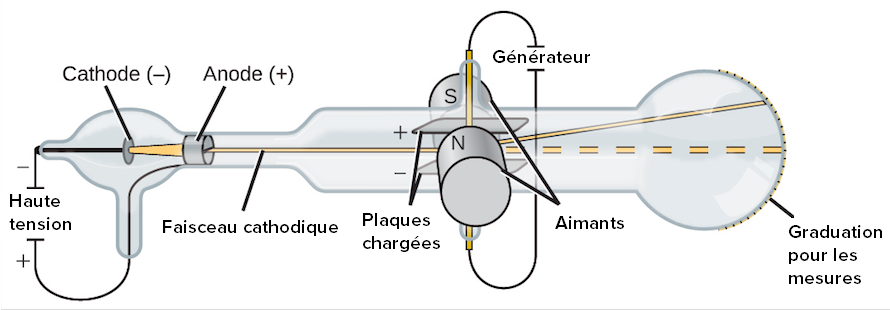
\includegraphics[scale=0.7]{images/02.JJ-Thomson.png}
    \caption{Maquette de l'expérience de Thomson}
    \label{fig:my_label}
\end{figure}
\begin{figure}[h!]
    \centering
    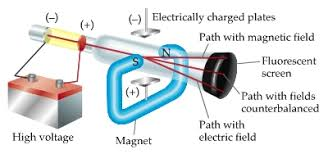
\includegraphics[scale=0.9]{images/08.JJ-Thomson..jpg}
    \caption{Autre schéma réaliste}
    \label{fig:my_label}
\end{figure}
Étapes du tube : \\
\begin{enumerate}
    \item générateur d'électrons
    \item cathode
    \item anode
    \item plaques métalliques chargées
    \item aimants
    \item écran fluorescent
\end{enumerate}
Tout d'abord, on a le générateur qui va générer/créer des électrons, vu que le tube a été mis sous vide, les électrons vont être attirés par la cathode (pas sûre). La cathode va les canaliser, puis ils vont passer à l'anode positive. Ils vont être canalisés en un faisceau cathodique.\\
Ce faisceau cathodique va ensuite passé entre deux plaques métalliques, celle au-dessus est chargée positivement et celle en-dessous est chargée négativement. Un générateur est Viennent ensuite deux aimants qui sont mis sur les côtés, à l'extérieur du tube, leur rôle est de ...(à chercher).\\
Après cela, si les électrons ont une vitesse assez élevée ils vont se diriger vers le haut, attirés par la plaque métallique positive. Si leur vitesse est au contraire assez basse ils vont se diriger vers le bas, attirés par la plaque métallique négative. Ou il y a la dernière catégorie, quand les électrons vont à la bonne vitesse, ils vont continuer tout droit à l'horizontale et vont être "taper" l'écran fluorescent. \\
Thomson a gradué son écran fluorescent qui est de force circulaire, en degrés pour comparer la vitesse des électrons au point où ils touchent l'écran. \\
Il a notamment pris des mesures sur les voltages des plaques métalliques, comme par exemple ceux des plaques métalliques. \\
On a également essayé de voir ce qu'il se passait quand on enlevait un seul élément voir même plusieurs, pour voir le changement que cela produirait et donc aussi voir si l'on parvenait quand même à atteindre le but final.

\end{document}